\clearpage
\section{Frame choices in special DH geometries}
\label{sec:l10-dh-special}
Many robot designs use parallel or perpendicular joint axes. These
geometries simplify the mechanism but require choices that the generic
skew-axis construction does not determine uniquely. The goal is to make
those choices once, attach each frame to its link, and use the same
definitions throughout the calculation.

\subsection{Parallel, intersecting, and coincident axes}
For two distinct \emph{parallel axes}, infinitely many common normals
exist. Translating a common normal along the axes gives another valid
one. A convenient choice often places neighboring origins at the same
axial level, making the corresponding constant $d_i$ zero. Once chosen,
the frames must remain attached to their links; they are not reassigned
at every configuration to force a changing parameter to vanish.

Choosing the two positive $z$ directions alike gives $\alpha_i=0$.
Choosing them oppositely gives a twist of $\pi$ modulo $2\pi$. Both can
be valid, but the first generally produces simpler matrices.

For two \emph{intersecting, nonparallel axes}, the separation is zero,
so $a_i=0$. Their common-normal line passes through the intersection and
is perpendicular to both axes. There are two choices for the positive
$x_i$ direction along that line. Thus its \emph{sense} is free, not its
orientation in space: an arbitrary direction through the intersection
would not generally be perpendicular to both joint axes. The chosen
sense determines the sign of the twist $\alpha_i$.

For \emph{coincident axes}, any line perpendicular to the shared axis
and intersecting it can serve as a common normal. Its location and
direction must be chosen consistently with the link frames. The
separation again gives $a_i=0$; with aligned positive $z$ directions,
$\alpha_i=0$ as well. Axial displacement and rotation may still be present.

\begin{figure}[htbp]
\centering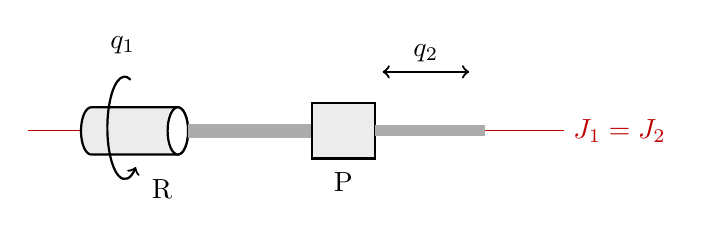
\begin{tikzpicture}
\draw[red!75!black] (-.8,0)--(6,0) node[right] {$J_1=J_2$};
\path[draw,thick,fill=gray!15] (0,-.3)--(1.1,-.3)
 arc[start angle=-90,end angle=90,x radius=.13,y radius=.3]
 --(0,.3) arc[start angle=90,end angle=270,x radius=.13,y radius=.3];
\draw[fill=white,thick] (1.1,0) ellipse (.13 and .3);
\draw[line width=5pt,gray!65] (1.23,0)--(2.8,0);
\draw[fill=gray!15,thick] (2.8,-.35) rectangle (3.6,.35);
\draw[line width=4pt,gray!65] (3.6,0)--(5,0);
\draw[<->,thick] (3.7,.75)--(4.8,.75) node[midway,above] {$q_2$};
\draw[->,thick] (.5,.65) arc[start angle=70,end angle=310,x radius=.22,y radius=.65];
\node[above] at (.4,.85) {$q_1$};
\node[below] at (.9,-.5) {R};
\node[below] at (3.2,-.4) {P};
\end{tikzpicture}

\caption{A revolute joint followed by a coaxial prismatic joint. Rotation
about the shared axis and translation along it are independent motions,
even though the two joint axes occupy the same line.}
\label{fig:l10-dh-coaxial}
\end{figure}

Coaxial R and P joints retain two independent coordinates, an angle and a
displacement. Two ideal coaxial R joints can also exist, but their
downstream orientation depends on the sum of their angles when the
positive directions agree. They are redundant for that downstream
kinematic effect; this does not make the two physical joints identical.

\subsection{Base and terminal frames}
Frame 0 has $z_0$ along $J_1$. Choose $O_0$ on that axis and choose a
perpendicular $x_0$. For a fixed base, this frame stays fixed while the
first moving link rotates. Aligning $x_0$ with a link in one configuration
does not make the first joint angle identically zero.

At the terminal link there is no physical $J_{n+1}$. Placing $O_n$ at
the tool point makes the final translation column directly useful.
The line through $O_n$ in the $x_n$ direction must intersect and be
perpendicular to $J_n$ for the standard DH construction. If $O_n$ is off
$J_n$, this selects the normal through that point. If $O_n$ is on $J_n$,
any perpendicular direction through it can be chosen. Then choose $z_n$
perpendicular to $x_n$; taking it parallel and equally directed to
$z_{n-1}$ often sets $\alpha_n=0$.

A required tool orientation need not obey these convenient choices.
In that case, retain a valid terminal DH frame and append the fixed tool
transformation. Changing a base or terminal frame changes the coordinates
reported by the model, even though the physical robot is the same.

\section{DH example: a planar RR arm}
\label{sec:l10-dh-rr}
Consider two revolute joints with parallel axes, followed by a tool at
the end of the second link. The link lengths are $\ell_1$ and $\ell_2$.
There are two joints, three frames, one common normal between the physical
joint axes, and two rows in the DH table.

\begin{figure}[htbp]
\centering\begin{tikzpicture}[scale=1.3]
\definecolor{dhbase}{RGB}{30,150,65}
\definecolor{dhone}{RGB}{155,65,180}
\definecolor{dhtool}{RGB}{225,115,20}
\coordinate (O) at (0,0);
\coordinate (A) at (3.35,.42);
\coordinate (B) at (4.95,2.22);
% Joint axes, selected common normal, and two alternative levels.
\draw[red!75!black] (-.3,-.81)--(.7,1.9) node[above] {$J_1$};
\draw[red!75!black] (3.05,-.39)--(4.05,2.32) node[above] {$J_2$};
\draw[sensorframe,dashed] (-.245,-.665)--(3.105,-.245);
\draw[sensorframe,dashed] (.455,1.235)--(3.805,1.655);
% Solid mechanical links, followed by the cylindrical joint bodies.
\draw[line width=9pt,gray!65] (O)--(A)--(B);
\draw[line width=6pt,gray!12] (O)--(A)--(B);
\foreach \p in {O,A} {
 \begin{scope}[shift={(\p)}]
 \path[draw,thick,fill=gray!15] (-.3,-.11)--(-.09,.46)
 arc[start angle=160,end angle=-20,x radius=.245,y radius=.12]
 --(.16,-.27) arc[start angle=-20,end angle=-200,x radius=.245,y radius=.12];
 \draw[fill=white,thick,rotate around={-20:(.12,.38)}] (.12,.38) ellipse (.245 and .12);
 \end{scope}
}
\draw[thick] ($(B)+(-.18,.05)$)--($(B)+(-.03,.35)$)--($(B)+(.13,.23)$);
\draw[thick] ($(B)+(.16,-.11)$)--($(B)+(.33,.17)$)--($(B)+(.18,.23)$);
\draw[sensorframe,thick] (O)--node[below,sloped] {$\mathrm{CN}_1$}(A);
\draw[axis,dhbase] (O)--(.35,.95) node[left] {$z_0$};
\draw[axis,dhbase] (O)--(1,-.22) node[below right] {$x_0$};
\draw[axis,dhone] (A)--++(.35,.95) node[left] {$z_1$};
\draw[axis,dhone] (A)--++(1.1,.138) node[right] {$x_1$};
\draw[axis,dhtool] (B)--++(.35,.95) node[above left] {$z_2$};
\draw[axis,dhtool] (B)--++(.8,.9) node[right] {$x_2$};
\foreach \p in {O,A,B} {\fill (\p) circle (.035);}
\node[dhbase,left] at (O) {$O_0$};
\node[dhone,below] at ($(A)+(0,-.18)$) {$O_1$};
\node[dhtool,below right] at (B) {$O_2$};
\draw[<->] (.1,.84)--node[above,sloped] {$\ell_1$}(3.45,1.26);
\draw[<->] (4.9,.12)--node[below right] {$\ell_2$}(6.5,1.92);
\draw[projection] (O)--(1.25,.156);
\draw[->,red!75!black] (.72,-.158) .. controls (.85,-.12) and (.87,.02) .. (.82,.103);
\node[red!75!black] at (1.08,.03) {$q_1$};
\draw[projection] (A)--++(1.4,.175);
\draw[->,red!75!black] ($(A)+(.9,.113)$) .. controls (4.25,.8) and (4.04,.99) .. (3.91,1.05);
\node[red!75!black] at (4.35,1.03) {$q_2$};
\end{tikzpicture}

\caption{Perspective view of the planar RR arm, with cylindrical revolute
joints and the terminal tool. The selected common normal follows the
first link. Dashed alternatives illustrate the freedom to shift it along
the parallel axes. Frame 0 is fixed; frames 1 and 2 move with their links.}
\label{fig:l10-dh-rr}
\end{figure}

Choose $O_0$ at the first joint and $O_1$ at the second, at the same axial
level. Put $O_2$ at the tool point. Let all three $z$ axes point in the
same direction, normal to the plane of motion. Choose $x_1$ along the
first link toward the second joint, and $x_2$ along the second link toward
the tool. The fixed $x_0$ defines the zero of $q_1$.

With the joint zeros chosen to match the DH angles, $\theta_1=q_1$ and
$\theta_2=q_2$. The second angle is measured relative to the first link,
not relative to the base. Since the $z$ axes are equally directed and
there is no displacement along them, the table is
\begin{center}
\begin{tabular}{ccccc}
\toprule
$i$ & $\theta_i$ & $\alpha_i$ & $a_i$ & $d_i$\\
\midrule
1 & $q_1$ & $0$ & $\ell_1$ & $0$\\
2 & $q_2$ & $0$ & $\ell_2$ & $0$\\
\bottomrule
\end{tabular}
\end{center}
The column order is a presentation choice; the column labels determine
the meaning. The joint count determines the number of rows. Filling the
variable entries first helps prevent mistaking an angle that happens to
be zero in the drawing for a constant zero parameter.

\subsection{Local matrices and the complete product}
Write $c_i=\cos q_i$, $s_i=\sin q_i$,
$c_{12}=\cos(q_1+q_2)$, and $s_{12}=\sin(q_1+q_2)$.
Each local matrix is a $z$ rotation followed by a translation along the
rotated $x$ axis:
\[
 H_1^0=\begin{bmatrix}
 c_1&-s_1&0&\ell_1c_1\\s_1&c_1&0&\ell_1s_1\\
 0&0&1&0\\0&0&0&1
 \end{bmatrix},\qquad
 H_2^1=\begin{bmatrix}
 c_2&-s_2&0&\ell_2c_2\\s_2&c_2&0&\ell_2s_2\\
 0&0&1&0\\0&0&0&1
 \end{bmatrix}.
\]
Their product is
\begin{equation}
 H_2^0=\begin{bmatrix}
 c_{12}&-s_{12}&0&\ell_1c_1+\ell_2c_{12}\\
 s_{12}&c_{12}&0&\ell_1s_1+\ell_2s_{12}\\
 0&0&1&0\\0&0&0&1
 \end{bmatrix}.
 \label{eq:l10-dh-rr}
\end{equation}
The translation column reproduces the geometric result in
Equation~\eqref{eq:l10-planar}, and the tool yaw is $q_1+q_2$.
DH has provided a systematic route to the same answer.

As a quick check, with $\ell_1=1\,\mathrm m$, $\ell_2=0.5\,\mathrm m$,
$q_1=0$, and $q_2=\pi/2$, the tool is at
$(1,0.5,0)\,\mathrm m$ and its $x_2$ axis points along $y_0$.
At $q_1=q_2=0$, the arm extends along $x_0$ to
$(\ell_1+\ell_2,0,0)$.

\section{DH example: a spatial RRP arm}
\label{sec:l10-dh-rrp}
The next arm has two revolute joints and one prismatic joint. The first
axis is vertical. The second intersects it at a height $\ell_1$ and is
perpendicular to it. The prismatic axis intersects the second joint axis
at a distance $\ell_2$ along that axis. The tool moves along the prismatic
axis. These are three joints and require four frames and three DH rows.

\begin{figure}[htbp]
\centering\begin{tikzpicture}[scale=1.3]
\definecolor{dhbase}{RGB}{30,150,65}
\definecolor{dhone}{RGB}{225,115,20}
\definecolor{dhtwo}{RGB}{155,65,180}
\definecolor{dhthree}{RGB}{195,65,120}
% Consistent oblique projection: X=(1,.1), Y=(-.8,.4), Z=(0,1).
% Shown at q1=pi, q2=0, l1=3, l2=3.5, q3=1.5 (drawing units).
\coordinate (O) at (0,0);
\coordinate (A) at (0,3);
\coordinate (B) at (2.8,1.6);
\coordinate (T) at (2.8,3.1);
\draw[red!75!black] (0,-.3)--(0,4.1) node[above] {$J_1$};
\draw[red!75!black] (-1.2,3.6)--(3.8,1.1) node[right] {$J_2$};
\draw[red!75!black] (2.8,.6)--(2.8,4.1) node[above] {$J_3$};
% Base revolute joint and upright support.
\draw[line width=6pt,gray!60] (0,.4)--(A);
\path[draw,thick,fill=gray!15] (-.35,.9)--(-.35,1.8)
 arc[start angle=180,end angle=0,x radius=.35,y radius=.12]
 --(.35,.9) arc[start angle=0,end angle=-180,x radius=.35,y radius=.12];
\draw[fill=white,thick] (0,1.8) ellipse (.35 and .12);
% Second revolute joint and its link toward the slider assembly.
\draw[line width=8pt,gray!70] (A)--(B);
\draw[line width=5pt,gray!15] (A)--(B);
\begin{scope}[shift={(A)},rotate=-26.565]
\path[draw,thick,fill=gray!15] (-.45,-.23)--(.55,-.23)
 arc[start angle=-90,end angle=90,x radius=.12,y radius=.23]
 --(-.45,.23) arc[start angle=90,end angle=270,x radius=.12,y radius=.23];
\draw[fill=white,thick] (.55,0) ellipse (.12 and .23);
\end{scope}
% Prismatic block, shaft, and terminal gripper.
\path[draw,thick,fill=gray!15] (2.45,1.25)--(3.05,1.15)--(3.05,1.8)--(2.45,1.9)--cycle;
\path[draw,thick,fill=white] (2.45,1.9)--(2.72,2.1)--(3.32,2)--(3.05,1.8)--cycle;
\path[draw,thick,fill=gray!30] (3.05,1.15)--(3.32,1.35)--(3.32,2)--(3.05,1.8)--cycle;
\draw[line width=5pt,gray!70] (B)--(T);
\draw[thick] (2.55,3.1)--(2.6,3.4)--(2.72,3.25);
\draw[thick] (3.05,3.1)--(3,3.4)--(2.88,3.25);
\draw[<->,thick] (3.65,1.85)--(3.65,2.65) node[midway,right] {P};
% Common normals through the intersecting joint axes.
\draw[sensorframe] (-1.25,2.875)--(1.05,3.105);
\node[sensorframe,above] at (1.05,3.2) {$\mathrm{CN}_1$};
\draw[sensorframe] (1.5,1.47)--(4.05,1.725) node[right] {$\mathrm{CN}_2$};
\draw[axis,dhbase] (O)--(0,.65) node[below left] {$z_0$};
\draw[axis,dhbase] (O)--(1.3,.13) node[right] {$x_0$};
\draw[axis,dhone] (A)--++(-1,-.1) node[below] {$x_1$};
\draw[axis,dhone] (A)--++(.8,-.4) node[below] {$z_1$};
\draw[axis,dhtwo] (B)--++(-1,-.1) node[left] {$x_2$};
\draw[axis,dhtwo] (B)--++(0,.95) node[left] {$z_2$};
\draw[axis,dhthree] (T)--++(-1,-.1) node[left] {$x_3$};
\draw[axis,dhthree] (T)--++(0,.7) node[left] {$z_3$};
\foreach \p in {O,A,B,T} {\fill (\p) circle (.035);}
\node[dhbase,below left] at (O) {$O_0$};
\node[dhone,above left] at (A) {$O_1$};
\node[dhtwo,below left] at (B) {$O_2$};
\node[dhthree,right] at (T) {$O_3$};
\draw[<->] (-1.7,0)--node[left] {$\ell_1$}(-1.7,3);
\draw[projection] (O)--(-1.8,0);
\draw[projection] (A)--(-1.8,3);
\draw[<->] (.2,4.25)--node[above,sloped] {$\ell_2$}(3,2.85);
\draw[projection] (A)--(.2,4.25);
\draw[projection] (B)--(3,2.85);
\draw[<->] (4.35,1.6)--node[right] {$q_3$}(4.35,3.1);
\draw[projection] (B)--(4.45,1.6);
\draw[projection] (T)--(4.45,3.1);
\end{tikzpicture}

\caption{The spatial RRP arm. The two cylinders represent revolute joints;
the block and sliding shaft represent the prismatic joint. Both neighboring
joint-axis pairs intersect, so their common normals pass through the
intersections. This illustrative configuration has $q_1=\pi$, $q_2=0$,
and $q_3>0$: the prismatic axis is vertical here but tilts when joint 2
rotates. Frames use distinct colors for readability.}
\label{fig:l10-dh-rrp}
\end{figure}

\subsection{Frames, signs, and the DH table}
Place frame 0 below the intersection of $J_1$ and $J_2$, with $z_0$
upward. Put $O_1$ at that intersection and choose $z_1$ along $J_2$
toward the prismatic assembly. Put $O_2$ where $J_2$ meets $J_3$, with
$z_2$ along the positive prismatic motion. Finally, put $O_3$ at the tool,
with $z_3=z_2$ and $x_3=x_2$ in direction.

At each intersection, choose the common-normal sense so that the twists
are $\alpha_1=-\pi/2$ and $\alpha_2=+\pi/2$. The first is the rotation
from $z_0$ to $z_1$ about $x_1$; the second is from $z_1$ to $z_2$ about
$x_2$. Both have magnitude $90^\circ$, but their signs differ. Use the
right-hand rule around the named positive $x$ axis, rather than the
apparent angle on the page.

Because the joint axes intersect, $a_1=a_2=0$. The tool origin lies on
the prismatic axis, so $a_3=0$ too. These zeros do not mean that the
physical links have zero length: $\ell_1$ and $\ell_2$ enter as offsets
along $z_0$ and $z_1$. Define $q_3$ as the signed tool displacement from
$O_2$ along $z_2$, with no additional zero offset. Then
\begin{center}
\begin{tabular}{cccccc}
\toprule
$i$ & Type & $\theta_i$ & $\alpha_i$ & $a_i$ & $d_i$\\
\midrule
1 & R & $q_1$ & $-\pi/2$ & $0$ & $\ell_1$\\
2 & R & $q_2$ & $+\pi/2$ & $0$ & $\ell_2$\\
3 & P & $0$ & $0$ & $0$ & $q_3$\\
\bottomrule
\end{tabular}
\end{center}
The revolute coordinates are angles; $q_3$ is a length. The last row has
$\theta_3=0$ because the terminal axes have been aligned with frame 2,
not because the third joint is absent.

\subsection{Local transformations}
Using $c_i=\cos q_i$ and $s_i=\sin q_i$ for $i=1,2$, the three matrices are
\begin{align}
 H_1^0&=\begin{bmatrix}
 c_1&0&-s_1&0\\s_1&0&c_1&0\\0&-1&0&\ell_1\\0&0&0&1
 \end{bmatrix},\\
 H_2^1&=\begin{bmatrix}
 c_2&0&s_2&0\\s_2&0&-c_2&0\\0&1&0&\ell_2\\0&0&0&1
 \end{bmatrix},\\
 H_3^2&=\begin{bmatrix}
 1&0&0&0\\0&1&0&0\\0&0&1&q_3\\0&0&0&1
 \end{bmatrix}.
\end{align}
The last matrix is a pure translation. Increasing $q_3$ moves the tool
along $z_2$ without changing its orientation relative to link 2.

\subsection{Complete direct kinematics and geometric checks}
Multiplication yields
\begin{equation}
 H_3^0=\begin{bmatrix}
 c_1c_2&-s_1&c_1s_2&-\ell_2s_1+q_3c_1s_2\\
 s_1c_2&c_1&s_1s_2&\ell_2c_1+q_3s_1s_2\\
 -s_2&0&c_2&\ell_1+q_3c_2\\
 0&0&0&1
 \end{bmatrix}.
 \label{eq:l10-dh-rrp}
\end{equation}
Its translation can also be assembled as three physical displacements,
all expressed in frame 0:
\begin{equation}
 p_3^0=
 \ell_1\begin{bmatrix}0\\0\\1\end{bmatrix}
 +\ell_2\begin{bmatrix}-s_1\\c_1\\0\end{bmatrix}
 +q_3\begin{bmatrix}c_1s_2\\s_1s_2\\c_2\end{bmatrix}.
 \label{eq:l10-dh-rrp-position}
\end{equation}
The middle vector follows the second joint axis. Rotation about that
axis changes the prismatic direction but does not change the position
of $O_2$, which lies on the rotation axis itself. The final unit vector
is also the third column of $R_3^0$, the tool's $z$ direction.

For $q_2=0$, the prismatic direction is vertical and
\[
 p_3^0=\begin{bmatrix}-\ell_2\sin q_1\\
 \ell_2\cos q_1\\\ell_1+q_3\end{bmatrix}.
\]
For $q_2=\pi/2$, it is horizontal, so changing $q_3$ leaves the tool
height equal to $\ell_1$. These limiting cases check both the signs and
the assignment of the prismatic coordinate.

For example, let $\ell_1=0.6\,\mathrm m$, $\ell_2=0.4\,\mathrm m$,
$q_1=0$, $q_2=\pi/2$, and $q_3=0.3\,\mathrm m$. Then
\[
 H_3^0=\begin{bmatrix}
 0&0&1&0.3\\0&1&0&0.4\\-1&0&0&0.6\\0&0&0&1
 \end{bmatrix}.
\]
The tool is at $(0.3,0.4,0.6)\,\mathrm m$ and its positive $z_3$
direction is $+x_0$. Increasing the extension by $0.1\,\mathrm m$
therefore increases only its $x_0$ coordinate by $0.1\,\mathrm m$.

\subsection{Checking a completed DH model}
A useful check is to distinguish geometry constants from joint variables.
An axis alignment visible in one drawing may disappear when a joint
moves. Conversely, the twist between adjacent joint axes is a fixed
property of the intervening rigid link in these models.

Check that there is one table row per joint, that each row contains the
correct variable parameter, and that translations are signed projections.
Then test a simple configuration against the robot drawing. If a different
valid frame assignment gives a different table, compare the resulting
poses only after expressing them in the same base and tool frames and
accounting for any changes in the joint zeros or positive directions.
